
% Voeg hier je eigen hoofdstukken toe die de ``corpus'' van je bachelorproef
% vormen. De structuur en titels hangen af van je eigen onderzoek. Je kan bv.
% elke fase in je onderzoek in een apart hoofdstuk bespreken.
\chapter{\IfLanguageName{dutch}{Case Study}{Managed service provider}}
\label{ch:corpus}

\section{Patching vermijden}

Volgens \textcite{Munck2024} kan patching volledig worden vermeden door een cloud service bij de ERP provider aan te schaffen. Zo kan men een cloud service aankopen zoals SAP RISE, Oracle Cloud ERP of Workday waarbij de 
managed service provider het patchwerk voor de klant gaan doen. In vele gevallen is de kostprijs van cloudservices voorspelbaarder en zeker in vergelijking met de lokale opslag. Vele bedrijven
 willen dit echter niet doen omwille van verschillen redenen.\\


\section{Waarom kiezen bedrijven voor lokale opslag?}
Ondanks de vele voordelen van cloud systemen kiezen sommige bedrijven nog voor lokale opslag. Vaak is de hoofdreden dat sommige services niet volledig worden ondersteund door standaard cloudoplossingen. Als bedrijf ben je dan ook afhankelijk van deze cloud provider en mocht er iets mislopen met de cloud provider kan dit grote gevolgen hebben voor het bedrijf.
In sectoren zoals overheid, gezondheidszorg en financiële dienstverlening speelt dataveiligheid en compliance een cruciale rol. Dit is ook vaak gemakkelijker te realiseren in een lokale omgeving.\\ 
In sommige gevallen hebben organisaties al aanzienlijk geïnvesteerd in lokale infrastructuur, waardoor de overstap naar de cloud kostbaar kan zijn en voor hun niet de moeite meer is.
Verder bieden lokale implementaties vaak meer flexibiliteit en controle over configuratie en aanpassingen, waardoor organisaties beter kunnen inspelen op hun specifieke behoeften en 
bedrijfsprocessen.\\



\section{Huidige situatie van het patchproces binnen een ERP Managed Service Provider bedrijf}

Er wordt in dit onderzoek gefocussed op systemen die door MSP's beheerd worden, lokaal of in de cloud. In figuur 1 (groot in Bijlage~\ref{bijlage:1}) is de 
huidige situatie van het patchproces te vinden binnen een ERP Managed Service Provider. \\

\begin{figure}[h]
    \centering
    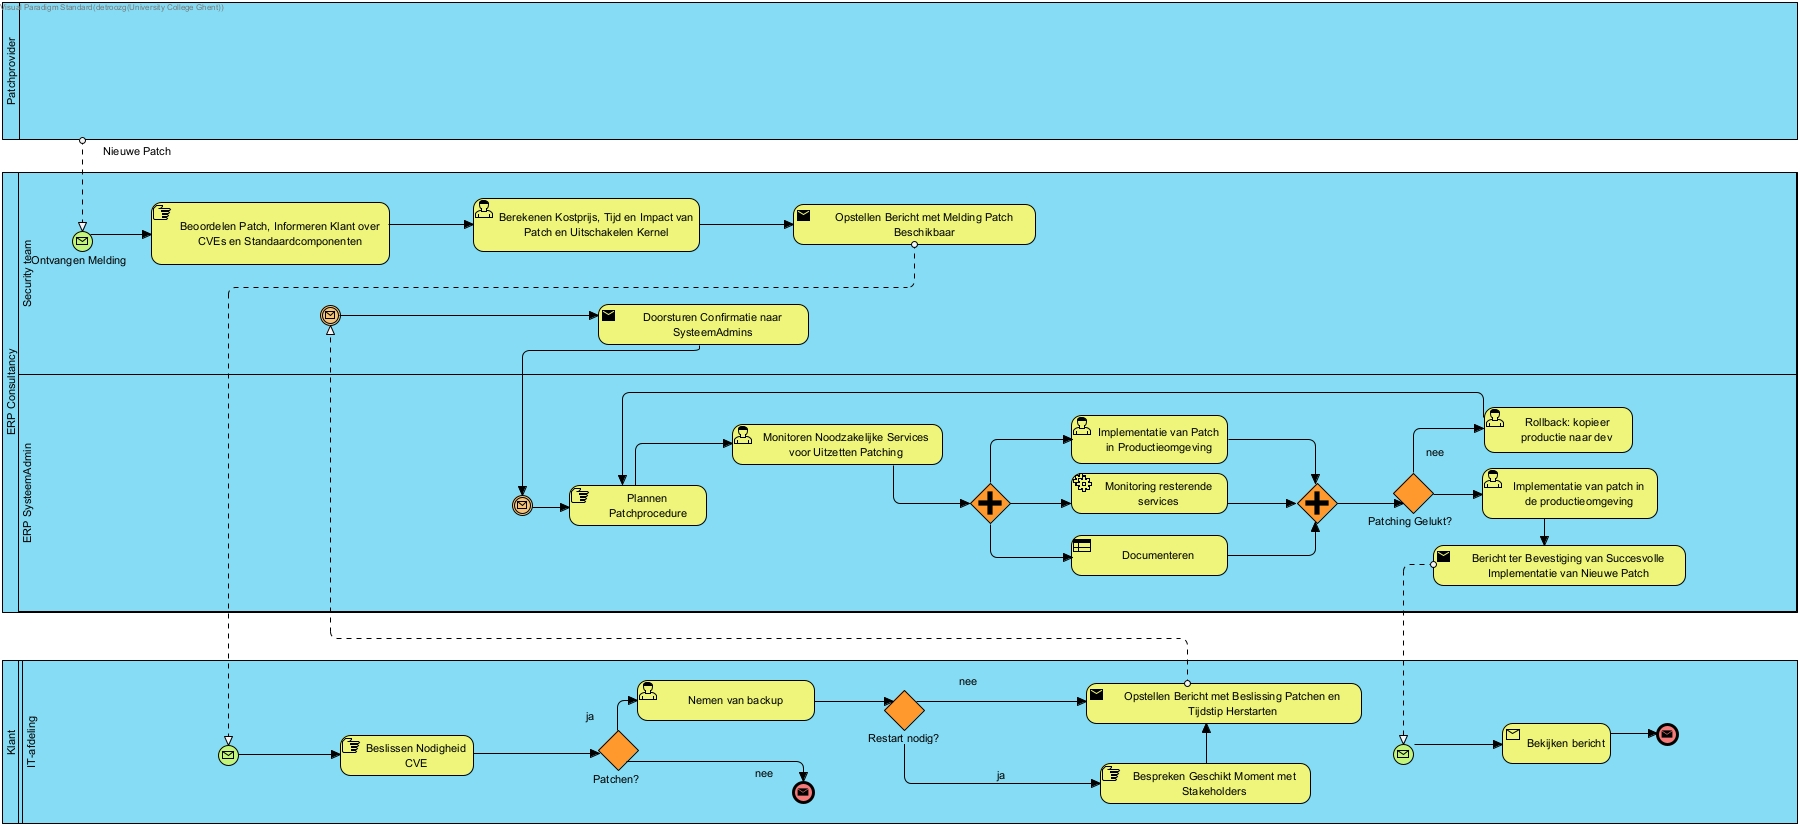
\includegraphics[width=\textwidth]{huidigesituatie.jpg}
    \caption{Huidige situatie (in het groot te zien in bijlage 1)}
    \label{fig:huidigesituatie}
\end{figure}
\newpage

Wat we dus kunnen afleiden uit het BPMN schema ~\ref{fig:huidigesituatie}, is dat communicatie van essentieel belang is, net omdat het zo belangrijk is, is het essentieel dat de communicatie tussen alle stakeholders zo vlot mogelijk verloopt. Dit kan door duidelijk en bondig te communiceren. Wat 
ook zeer belangrijk onderdeel is, is het actief luisteren naar de klant hun noden. Dit kan bijvoorbeeld zijn de tijdsspanne waarin ze willen patchen, of op voorhand afspreken
 welke patches mogen uitgevoerd worden door de managed service provider zonder de uitdrukkelijke toestemming van de klant. Nog een belangrijke communicatie is de klant informeren wanneer de patch gaat worden uitgevoerd en de wanneer deze uitgevoerd is om zo geen paniek te zaaien bij de klant. 

 Met de opkomst van AI (artificiële intelligentie) zal het communiceren alleen maar sneller en efficiënter verlopen. Zo kan AI bijvoorbeeld de agenda raadplegen en automatisch een tijdstip voorstellen voor de patch. Ook zou een AI kunnen helpen met een 
prioriteit toe te kennen aan een patch om zo te bepalen wanneer een bepaalde patch zal moeten worden geïntegreerd met gevolg dat het proces nog verder meer zal versnellen. \\

Voor het patchen zelf bieden patchproviders het nog niet aan om automatisch patches te kunnen downloaden er zal dus eerst manueel een patch moeten worden gedownload worden bij de ERP provider. Het patchingsproces begint met het beoordelen van de patch. Het security team bekijkt of het nut heeft
om te patchen, dit bepalen ze meestal door het type patch. Indien het een component patch of hotfix (= dringende patch) is zal dit een minder dringende patch zijn ten opzichte van een CVE (Common Vulnerabilities and Exposures) patch. De kostprijs, tijd en impact berekenen
die de patch nodig zal hebben zal verschillen van patch tot patch, maar volgens \textcite{Heyndrickx2024} zal een gemiddelde patching procedure van een kernel tussen 30 minuten en één uur duren per systeem, dit bevestigd nogmaals de nood aan
automatisatie van dit proces, zeker indien je meerdere systemen moet patchen per week. CVE's en hotfixes krijgen meestal een cijfer toegekend wat de urgentie van de patch aantoont. Indien dit een component patch is zal dit veel minder middelen kosten vergeleken
met een kernel patch bijvoorbeeld. Dit is zeer afhankelijk van situatie tot situatie dus hier kan men het proces niet verder worden geoptimaliseerd. In figuur ~\ref{fig:huidigesituatie} is er ook duidelijk te zien dat er veel gecommuniceerd moet worden tussen alle betrokken partijen, dit is dus een essentieel onderdeel van het patchmanagement. \\


\section{Waar kan er worden geoptimaliseerd?}

Het omkaderde deel in figuur 2 (groot in Bijlage~\ref{bijlage:2}) is waar het patchmanagement proces zelf zou kunnen worden geoptimaliseerd, de rest van het proces bestaat voornamelijk uit communicatie.
 \begin{figure}[h]
    \centering
    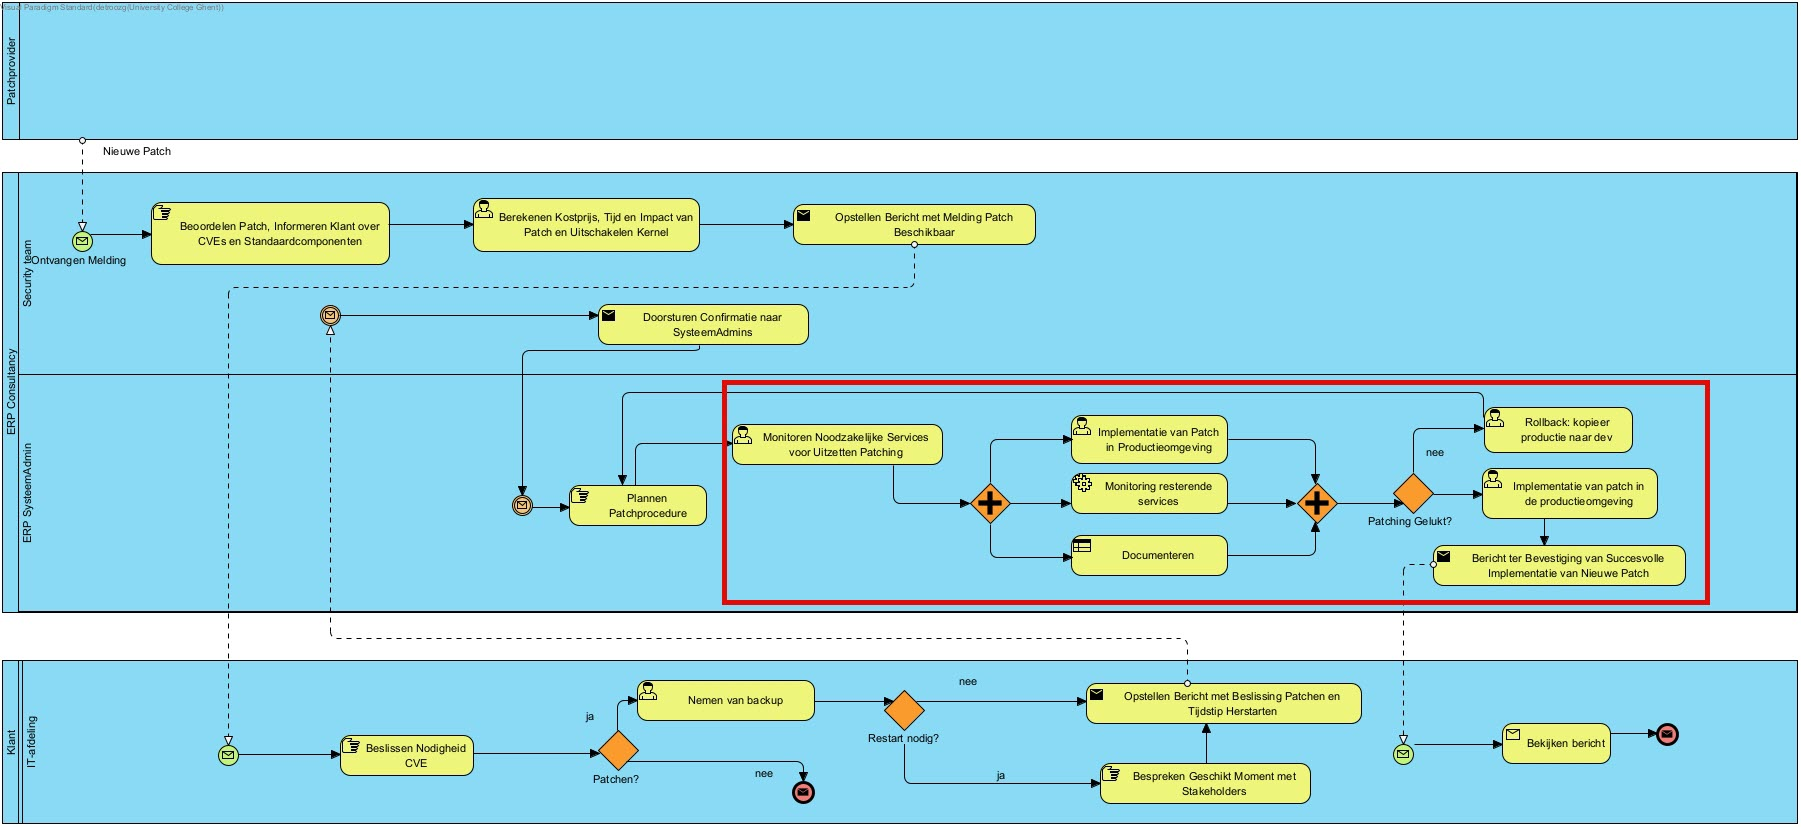
\includegraphics[width=\textwidth]{huidigesituatie2.jpg}
    \caption{Deel dat kan geautomatiseerd worden (=Patchen zelf)}
     \label{fig:huidigesituatie2}
\end{figure}
\newpage


Enkele tools die kunnen worden gebruikt voor een kernel patch van een ERP systemen zijn Avantra, SAP Landscape Management (LaMa) en SolarWinds Patch Manager. Deze tools bieden diverse voordelen en nadelen, afhankelijk van de specifieke behoeften van een organisatie. \\
 Avantra is specifiek gericht op SAP-systemen, waardoor het makkelijker wordt voor de gebruiker om zijn SAP systeem hiermee te koppelen en te configureren. Avantra biedt geautomatiseerde patchmanagementprocessen voor kernel patches en real-time monitoring, maar heeft 
  beperkte functionaliteit voor niet-SAP-systemen. Nog voor SAP systemen is SAP Landscape Management nog een alternatief. Deze software minder gebruiksvriendelijk, er is dus een steile leercurve voor beginnende gebruikers. Het voordeel 
 bij LaMa is dat je niet alleen kernel patching kan doen maar ook database patching vat niet het geval is bij Avantra. \\
 SolarWinds Patch Manager heeft een eenvoudige implementatie en gebruiksvriendelijke interface, geschikt voor kleine tot middelgrote bedrijven. Het biedt ondersteuning voor een breed scala aan 
 systemen, maar heeft mogelijk beperkte automatiseringsmogelijkheden. \\

 Voor niet-SAP-systemen zou SolarWinds Patch Manager een goede keuze kunnen zijn. Het biedt een breed scala aan ondersteunde besturingssystemen en softwareapplicaties, waardoor het geschikt is voor
  een diverse IT-infrastructuur. Bovendien staat SolarWinds bekend om zijn gebruiksvriendelijke interface en eenvoudige implementatie, wat vooral handig kan zijn voor organisaties die geen gespecialiseerde IT-vaardigheden hebben.
 
Voor SAP systemen zou Avantra een goede keuze zijn voor kernelpatching, doordat deze tool ook echt rond SAP is ontwikkeld. \\

\section{Nieuwe situatie}
\begin{figure}[h]
    \centering
    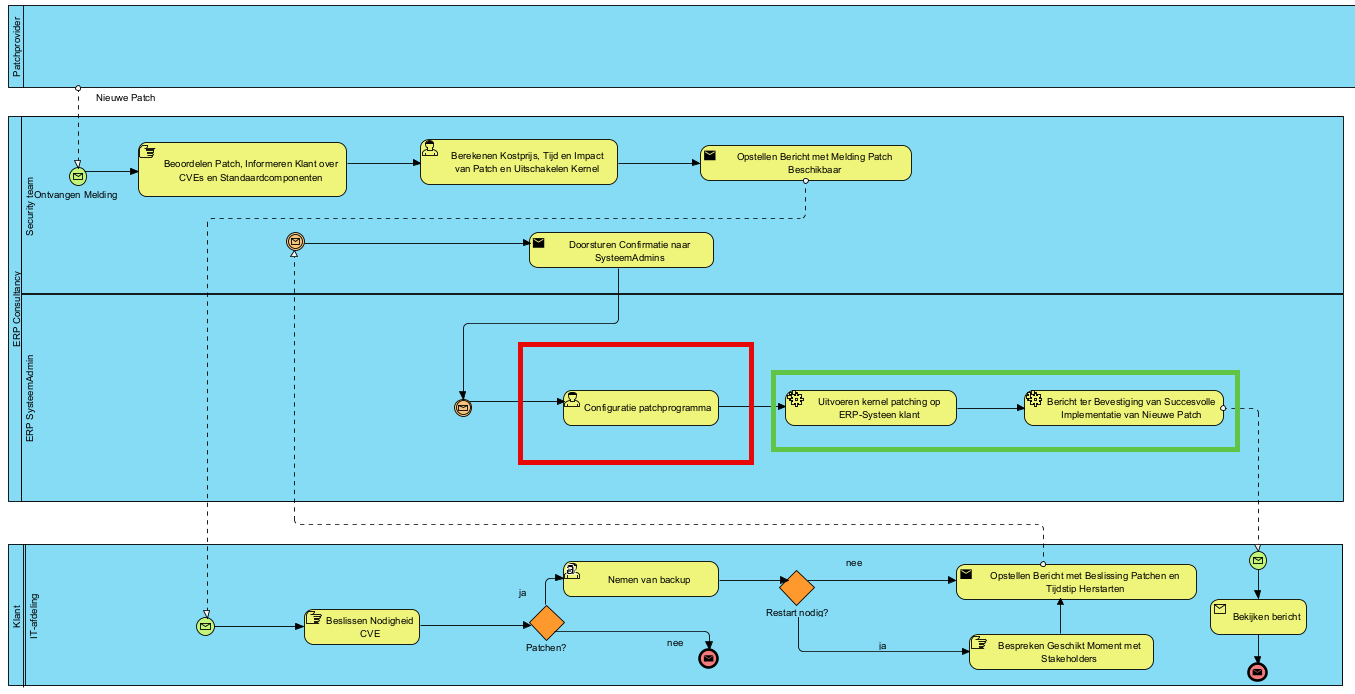
\includegraphics[width=\textwidth]{nieuwesituatie.png}
    \caption{Nieuwe Situatie: wanneer men patchautomatisatie toepast}
     \label{fig:nieuwesituatie}
\end{figure}
\newpage

In figuur ~\ref{fig:nieuwesituatie} is de situatie te zien wanneer we patchautomatisatie toepassen, er valt dus een groot deel van het proces weg. In het rood is het deel
waar men nog steeds manueel moet ingrijpen, dit is het deel waar de configuratie van het automatisatie programma gebeurt. In het groen is het de deel waar het programma de patching uitvoert. Dit was voordien een proces dat tussen de 30 minuten en 1 uur de volledige aandacht van de 
gebruiker vroeg. Dit zou nu in de achtergrond kunnen gebeuren en de gebruiker kan verder werken, en zo de efficiëntie dus verhogen. \\

\section{Avantra voor patchautomatisatie}
Doordat het grootste business netwerk wereldwijd door het SAP systeem beheerd wordt \autocite{Laborde2024} en het bedrijf waar de case study van is uitgevoerd enkel gebruik maakt van SAP systemen, focust deze studie zich verder op het gebruik van Avantra voor kernel patching.

\begin{figure}[h]
    \centering
    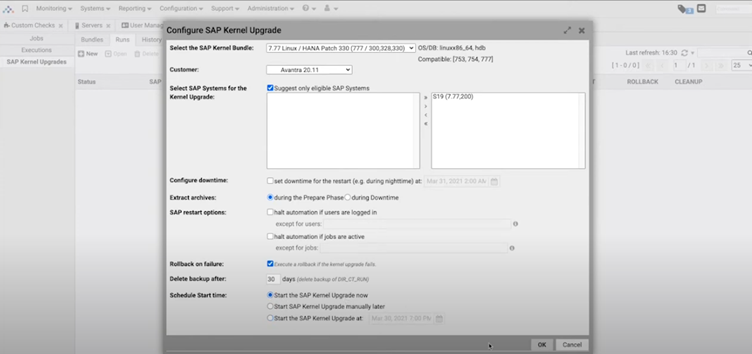
\includegraphics[width=\textwidth]{avantra1.png}
    \caption{Avantra patch configuratie}
     \label{fig:avantra1}
\end{figure}
\newpage


Binnen de software worden alle fasen van het proces worden duidelijk vermeld en er wordt er bevestiging gegeven indien de fase correct verlopen is. In de figuur ~\ref{fig:avantra1} zien we dat Avantra verschillende
nuttige functies heeft zoals een back-up maken van de huidige staat, bericht sturen naar de gebruikers om de real time status weer
   te geven, het systeem automatisch naar beneden halen, indien nodig een rollback uitvoeren met de voorgaande back-up die werd gemaakt enzovoort. Het proces kan op een zeer eenvoudige manier worden opgevolgd zoals te zien in figuur ~\ref{fig:avantra2}. Hier zien we op een duidelijk in welke fase het patchingsproces zit en kunnen we het zo opvolgen indien we wensen.\\

\begin{figure}[h]
    \centering
    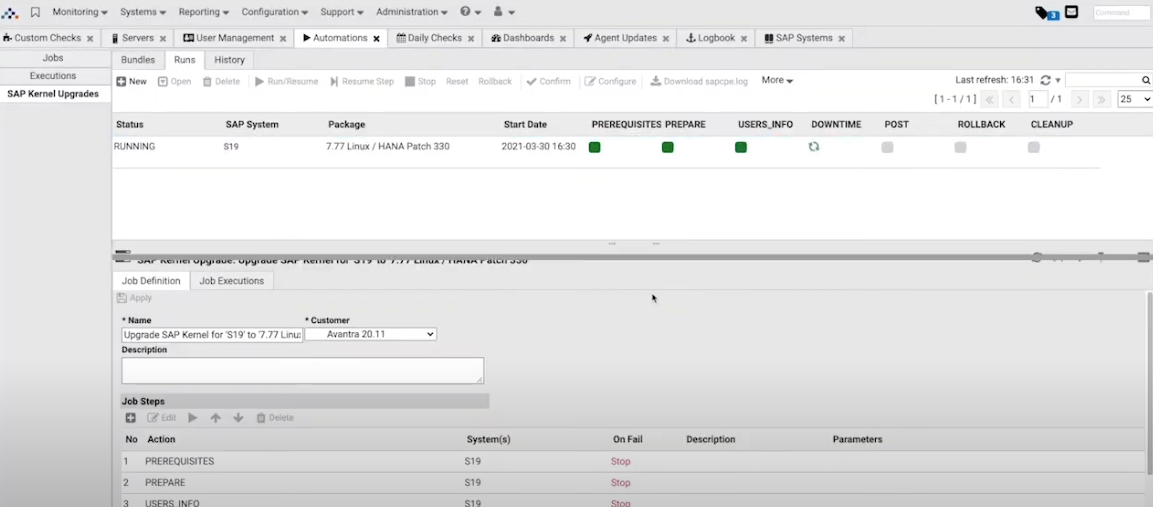
\includegraphics[width=\textwidth]{avantra2.png}
    \caption{Avantra patch configuratie detail}
     \label{fig:avantra2}
\end{figure}
\newpage

Berichten van het programma zoals error codes kunnen ook in meer detail worden bekeken zodat er kan gezien worden waar de fout zou zitten mocht er één zijn, zoals te zien is in figuur ~\ref{fig:avantra3}.

\begin{figure}[h]
    \centering
    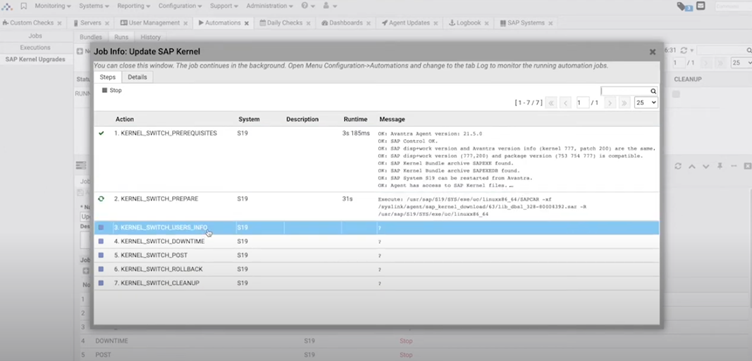
\includegraphics[width=\textwidth]{avantra3.png}
    \caption{Avantra patch configuratie}
     \label{fig:avantra3}
\end{figure}
\newpage


\subsubsection{Opstelling Avantra systeen}
Voor een automatisch patchmanagement moet men een omgeving opstellen, in figuur ~\ref{fig:avantra4} staat een mogelijk opstelling voor een Avantra systeem. 
\begin{figure}[h]
    \centering
    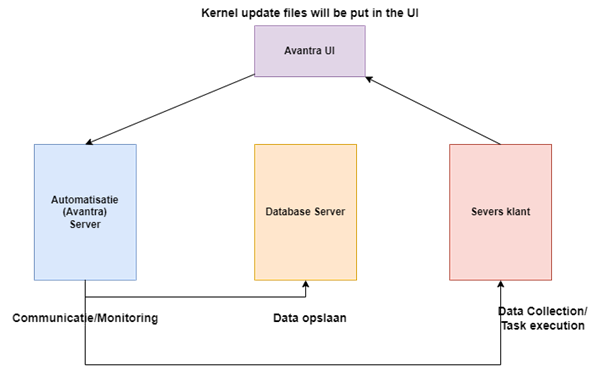
\includegraphics[width=\textwidth]{avantra4.png}
    \caption{Avantra opstelling van het systeem}
     \label{fig:avantra4}
\end{figure}
\newpage

De Avantra UI is de de interface waar de gebruikers effectief met communiceren, hierin staan alle functionaliteiten van het Avantra-Systeem. Zo kan bijvoorbeeld het SAP-systeem gemonitord worden. Op
dit platform zal de patchbeheerder de patch moeten uploaden en de configuratie instellen. De automatisatie server zorgt voor het uitvoeren van de geautomatiseerd taken en processen binnen de SAP-omgeving dit is dan ook het centrum van het Avantra systeem.
Vervolgens is er een Database server die relevante gegevens opslaat van de SAP-omgeving van de klant. Dit kan bijvoorbeeld informatie zijn over systeemconfiguraties, prestatiegegevens, logs, meldingen en historische trends. 

Tot slot integreert Avantra met de SAP-server van de klant, waar de SAP-applicaties draaien. Avantra maakt verbinding met deze server om real-time gegevens te verzamelen.
Op basis van deze gegevens kan Avantra proactief problemen identificeren, mogelijke risico's signaleren en eventueel automatisch acties ondernemen om de SAP-omgeving betrouwbaarder te maken.




\subsubsection{Voordelen van Avantra}
Wanneer Avantra wordt gestart ziet men een gebruiksvriendelijke design, op figuur ~\ref{fig:avantra4} staat een voorbeeld een patch configuratie. Bepaalde parameters worden ingegeven: bijvoorbeeld de bundle (type kernel en database), de downtime, backup of 
 rollback wil configureren. \\ 

\subsubsection{Nadelen van Avantra}
Avantra heeft dus vele voordelen maar ook nadelen. Zo is het een tool die enkel kernel patching doet en dus geen database patching, dit moet dan wel nog manueel worden gedaan. Ook is het een betalende tool en het bedrag kan hoog oplopen naarmate de grootte van het bedrijf.
En daarbij is het belangrijk om te weten dat een automatisatie geen plug en play is, er moeten enkele stappen worden ondernomen om het systeem op te stellen.

Zo is er een integratie van Avantra nodig in verschillende servers. In figuur ~\ref{fig:avantra4} staan de onderdelen van het Avantra opstelling. Bij deze opstelling komt dus vrij veel werk kijken.